\section{Results}
\label{sec:results}

\subsection{Embedding Validation}
\label{sec:results-sanity}

Before turning to substantive findings, we report two qualitative
sanity checks of the embedding.

The top-$10$ embedding-cosine nearest neighbors of São Paulo capital
($\text{IBGE} = 355030$) are: São Bernardo do Campo, Guarulhos, Diadema,
Taboão da Serra, Itaquaquecetuba, Embu das Artes, Santo André, Osasco,
Arujá, and Ferraz de Vasconcelos. All ten are members of the official
Greater São Paulo metropolitan area, ranging from cities directly
contiguous with the capital (Guarulhos, São Bernardo, Osasco) to
peripheral municipalities $30\text{--}50$\,km from the city center.

The top-$10$ neighbors of Manaus ($130260$) are: Careiro da Várzea,
Iranduba, Rio Preto da Eva, Presidente Figueiredo, Careiro, Novo Airão,
Codajás, Beruri, Caapiranga, and Manacapuru. These are the
ribeirinho municipalities reachable by river or short-haul air, all
formally inside the Manaus health region. Several (Codajás, Beruri,
Caapiranga) are between $150$ and $250$\,km of river distance from the
capital and have no road connection. The embedding correctly recovers
the Amazonian river-driven catchment.

In neither case did we engineer features that would have given the
embedding spatial information: the only input is the bipartite admission
graph. The recovery of metropolitan and ribeirinho geography is an
emergent property of the patient-flow structure.

The Pearson correlation between municipality-pair embedding distance
and haversine distance, computed on $5{,}000$ random pairs, is
$\rho = 0.299$ (Spearman $0.209$). Figure \ref{fig:emb-vs-km}
visualizes the bivariate density and the binned median embedding
distance by km-percentile, showing that the relationship is monotonic
but saturating: pairs separated by more than roughly $1{,}500$\,km
are nearly always also distant in the embedding, but at moderate
geographic distances ($100\text{--}500$\,km) the embedding distance
spreads widely.

\begin{figure}[h!]
    \centering
    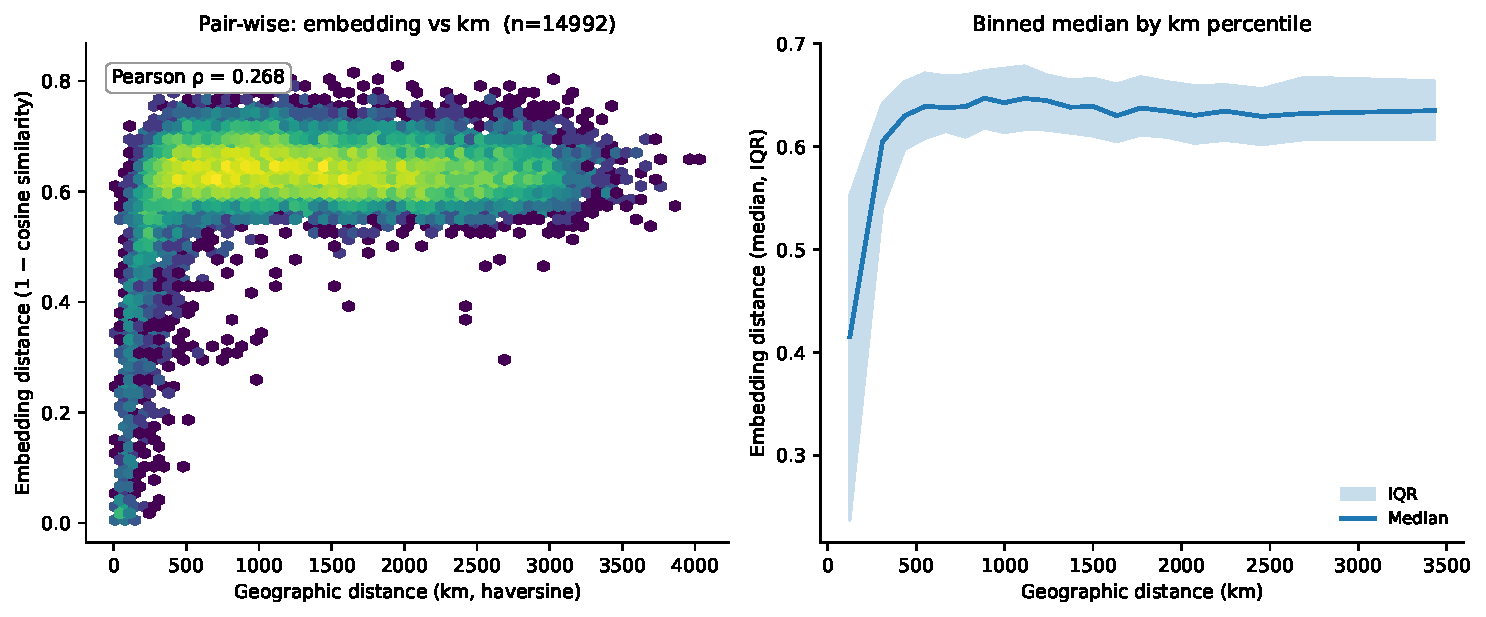
\includegraphics[width=0.95\textwidth]{../04_figures/fig_emb_vs_km.pdf}
    \caption{Embedding distance vs.\ haversine distance for $5{,}000$
    random municipality pairs. Left panel: hexbin density on a log
    color scale. Right panel: binned median (line) and IQR (shaded)
    of embedding distance across kilometer-percentile bins. The
    relationship is monotonic but saturating, leaving substantial
    embedding-distance variation orthogonal to geography at moderate
    physical distances.}
    \label{fig:emb-vs-km}
\end{figure} This moderate correlation is the
desired outcome: a value near $1$ would indicate that the embedding
contains no information beyond geography; a value near $0$ would
suggest the embedding has lost all spatial signal. The fact that
$1 - \rho^2 \approx 91\%$ of embedding-distance variance is orthogonal
to geography is the empirical opening for the divergence analysis.

\subsection{Two-Dimensional Visualization}
\label{sec:results-2d}

To assess the embedding's global structure beyond the two-pair sanity
check above, Figure \ref{fig:tsne-umap} projects the M-M embedding into
two dimensions using both t-SNE \citep{vandermaaten2008} and UMAP
\citep{mcinnes2018}, with each municipality coloured by its IBGE
macro-region. Recall that the embedding never sees coordinates: it is
constructed entirely from patient flow co-attendance.

Both projections separate the five macro-regions into distinguishable
clusters. The North forms a compact cluster reflecting the small
number of distinct Amazonian hospital catchments. The Southeast and
Northeast spread broadly, reflecting the large number of internal
hubs (capital tertiary hospitals plus inland regional hubs). Capital
anchors emerge as natural foci within their respective regional
clusters. The fact that this regional segregation emerges without
geographic input is the key qualitative evidence that the embedding
captures meaningful structure of the SUS hospital network.

\begin{figure}[h!]
    \centering
    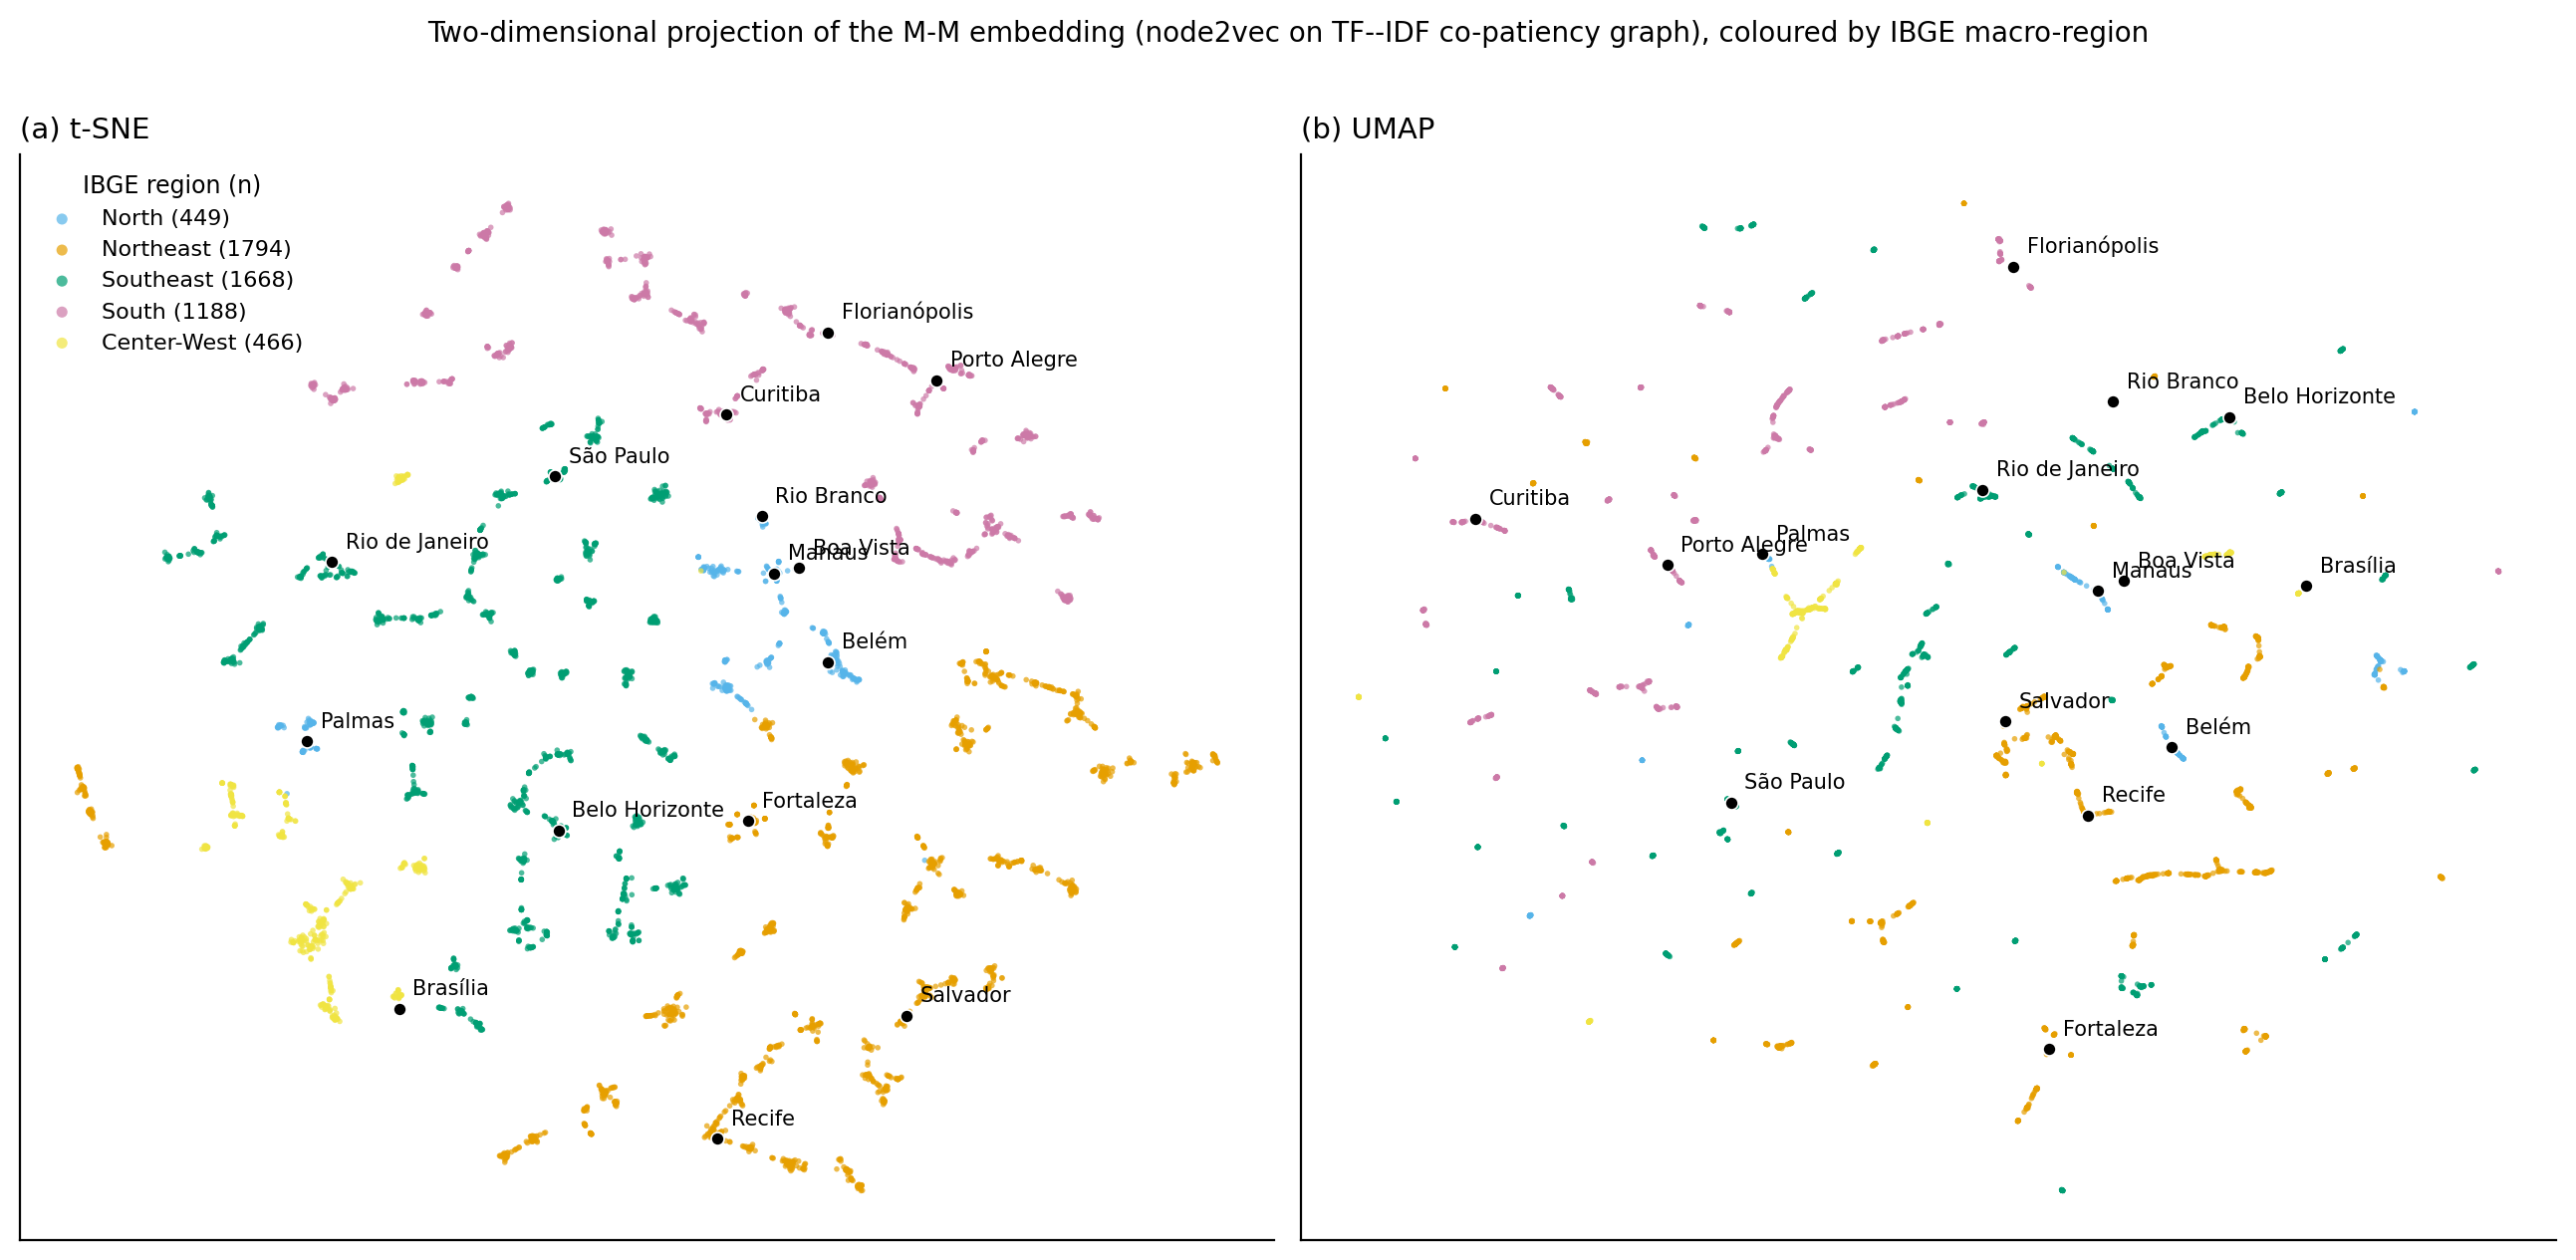
\includegraphics[width=0.99\textwidth]{../04_figures/fig_tsne_umap.png}
    \caption{Two-dimensional projection of the $128$-dimensional M-M
    embedding via (a) t-SNE (perplexity $30$, cosine metric) and
    (b) UMAP (\texttt{n\_neighbors=30}, $\min$-dist $0.1$, cosine).
    Each point is one municipality, coloured by IBGE macro-region.
    Black dots mark capital anchors. Both projections recover regional
    structure from patient-flow co-attendance alone, with no
    geographic input.}
    \label{fig:tsne-umap}
\end{figure}

\subsection{The Divergence Map}
\label{sec:results-divergence}

Figure \ref{fig:map-divergence} displays the divergence $\divz_m$ for
all $5{,}565$ Brazilian municipalities with both an embedding vector and
geographic coordinates. The cross-sectional standard deviation is
$0.91$, with the $5$th and $95$th percentiles at $-1.45$ and $+1.47$
respectively. The disagreement is large and geographically organized.

\begin{figure}[h!]
    \centering
    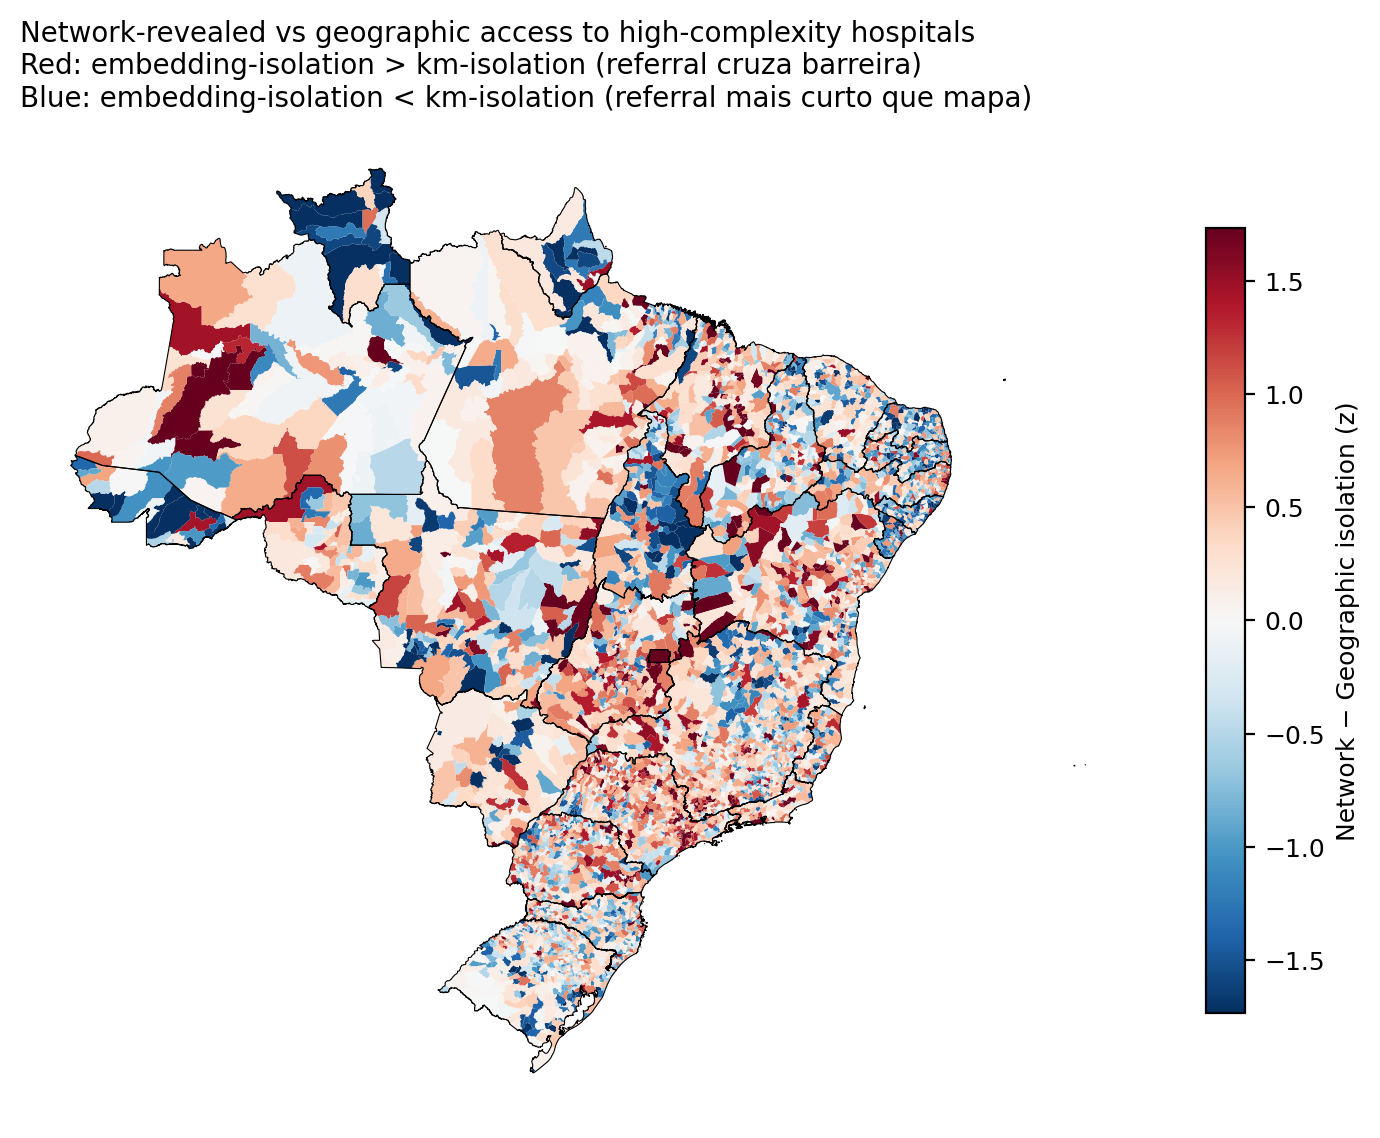
\includegraphics[width=0.85\textwidth]{../04_figures/fig_map_divergence.png}
    \caption{Network-revealed minus geographic isolation, by municipality.
    Red: embedding measures the municipality as more isolated than the
    map suggests, indicating that patients leapfrog the nominally
    nearest hospital. Blue: less isolated than the map suggests,
    indicating that the geography overstates isolation because patients
    reach a distant hub via channels (river, air) that road geography
    ignores. Color bar truncated at $\pm$ the $95$th absolute percentile.}
    \label{fig:map-divergence}
\end{figure}

\paragraph{Northern Brazil: river and air corridors.}
The Amazonian states---Amazonas, Roraima, Acre, Pará, Amapá, Rondônia,
Tocantins---show predominantly negative divergence. Median geographic
isolation in the North is $30$\,km (vs $14\text{--}19$\,km in the rest
of the country), but the embedding sees these municipalities as
considerably more connected than the kilometer figure suggests. The
canonical case is Caroebe-RR ($\divz = -2.91$): the nearest
high-complexity hospital is $210$\,km away by air, but the embedding
distance is $0.021$, deep in the lower tail. Pracuúba-AP
($\divz = -2.90$, $\isokm = 124$\,km), Amajari-RR ($\divz = -2.74$,
$\isokm = 203$\,km), Alto Alegre-RR ($\divz = -2.61$, $\isokm = 226$\,km),
and Uiramutã-RR ($\divz = -2.63$, $\isokm = 181$\,km) form a Roraima--
Amapá frontier cluster collectively reaching the Boa Vista, Manaus, and
Macapá hubs by air or boat. São Félix do Tocantins-TO
($\divz = -2.40$, $\isokm = 147$\,km) is a southern Tocantins case
where the patient flow tracks the Belém--Brasília highway corridor
beyond what road distance alone would predict. The road metric records the absence of land connection
mechanically; the embedding records that patients arrive nonetheless.

\paragraph{Northeastern semi-arid and Cerrado interior: bypassed local hospitals.}
The interior of Bahia, Maranhão, Piauí, and Goiás, together with
fragments of Minas Gerais and the Northern Cerrado, shows the opposite
pattern: dense red on the map, with positive divergence in
$541$ municipalities at $|\divz| > 1.0$. The canonical cases are
Bonito-BA ($\divz = +4.65$, $\isokm = 33$\,km, embedding distance
$0.268$), Jacutinga-MG ($\divz = +4.10$, $\isokm = 22$\,km), Vitorino
Freire-MA ($\divz = +3.90$, $\isokm = 32$\,km), Fronteiras-PI
($\divz = +3.57$, $\isokm = 38$\,km), and Iramaia-BA ($\divz = +3.45$,
$\isokm = 39$\,km). Two striking $\isokm = 0$\,km cases lie inside
high-density urban Brazil: Birigui-SP ($\divz = +3.19$) and
Brasília-DF ($\divz = +3.22$). In both, a high-complexity habilitation
exists at the residential location but the embedding records that
patients overwhelmingly reach their high-complexity care
elsewhere---in the Brasília case, in regional facilities just across
the GO/DF border serving capacity-saturated demand from the Federal
District. In all these cases the
nominally-nearest hospital is either too small to deliver the indicated
procedure, lacks active SUS habilitation in the relevant specialty, or
is bypassed by referral norms favoring regional capitals.

\paragraph{Southeast and Center-West: metropolitan saturation.}
The Southeast shows a moderately positive average divergence
($\bar{\divz}_{\text{SE}} = +0.19$), with the top quartile concentrated
in the Greater São Paulo periphery and Minas Gerais interior. This is
consistent with metropolitan-saturation logic: nominally-near tertiary
hospitals are operating at capacity, and incremental patients are
referred to second-tier hubs farther away. Center-West shows a similar
pattern at lower magnitude.

Tables \ref{tab:top15-pos} and \ref{tab:top15-neg} list the
canonical cases at each tail of the divergence distribution. They
make the spatial logic of the divergence transparent.

\begin{table}[ht]
\centering
\caption{Top-15 municipalities with highest positive divergence (network-revealed isolation exceeds geographic). The nominally nearest high-complexity hospital is bypassed.}
\label{tab:top15-pos}
\small
\begin{tabular}{llcrrr}
\toprule
IBGE-6 & Municipality & UF & km to nearest & emb dist & $\divz$ \\
\midrule
  290405 & Bonito & BA & 33 & 0.268 & +4.65 \\
  313490 & Jacutinga & MG & 22 & 0.238 & +4.10 \\
  211300 & Vitorino Freire & MA & 32 & 0.239 & +3.90 \\
  330460 & Santa Maria Madalena & RJ & 22 & 0.219 & +3.60 \\
  220430 & Fronteiras & PI & 38 & 0.230 & +3.57 \\
  521580 & Palmelo & GO & 4 & 0.177 & +3.46 \\
  291430 & Iramaia & BA & 39 & 0.226 & +3.45 \\
  500568 & Mundo Novo & MS & 28 & 0.218 & +3.43 \\
  130195 & Itamarati & AM & 233 & 0.266 & +3.38 \\
  522200 & Vianópolis & GO & 26 & 0.212 & +3.32 \\
  210380 & Dom Pedro & MA & 19 & 0.203 & +3.26 \\
  530010 & Brasília & DF & 0 & 0.129 & +3.22 \\
  350650 & Birigui & SP & 0 & 0.129 & +3.19 \\
  210790 & Passagem Franca & MA & 41 & 0.218 & +3.19 \\
  521400 & Mozarlândia & GO & 38 & 0.215 & +3.17 \\
\bottomrule
\end{tabular}
\medskip

\footnotesize
Notes: \textit{km to nearest} is the haversine distance to the nearest high-complexity hospital with an embedding vector. \textit{emb dist} is $1 - \cos$ to the same hospital under the embedding. $\divz$ is the standardized difference (Equation \ref{eq:divz}).
\end{table}

\begin{table}[ht]
\centering
\caption{Top-15 municipalities with most negative divergence (network-revealed isolation lies below the geographic). Geography overstates isolation because patients reach distant hubs via channels that road geography ignores (river, air, informal cross-border referral).}
\label{tab:top15-neg}
\small
\begin{tabular}{llcrrr}
\toprule
IBGE-6 & Municipality & UF & km to nearest & emb dist & $\divz$ \\
\midrule
  140023 & Caroebe & RR & 210 & 0.021 & -2.91 \\
  160055 & Pracuúba & AP & 124 & 0.009 & -2.90 \\
  510450 & Indiavaí & MT & 94 & 0.009 & -2.74 \\
  140002 & Amajari & RR & 203 & 0.027 & -2.74 \\
  140070 & Uiramutã & RR & 181 & 0.028 & -2.63 \\
  140005 & Alto Alegre & RR & 226 & 0.034 & -2.61 \\
  172015 & São Félix Do Tocantins & TO & 147 & 0.032 & -2.40 \\
  500310 & Corguinho & MS & 84 & 0.020 & -2.37 \\
  430543 & Chuí & RS & 66 & 0.016 & -2.34 \\
  510682 & Porto Esperidião & MT & 71 & 0.018 & -2.31 \\
  510160 & Barão De Melgaço & MT & 98 & 0.026 & -2.31 \\
  171270 & Mateiros & TO & 96 & 0.029 & -2.22 \\
  510380 & Figueirópolis D'oeste & MT & 81 & 0.026 & -2.19 \\
  510835 & Vale De São Domingos & MT & 80 & 0.026 & -2.18 \\
  353220 & Narandiba & SP & 49 & 0.015 & -2.18 \\
\bottomrule
\end{tabular}
\medskip

\footnotesize
Notes: see Table \ref{tab:top15-pos}.
\end{table}


\paragraph{The South: a calibrated benchmark.}
Paraná, Santa Catarina, and Rio Grande do Sul exhibit the smallest
absolute divergence ($\bar{\divz}_{\text{S}} = -0.10$, cross-sectional
$\mathrm{sd} = 0.77$, the lowest of all regions). The geography of
nearest-hospital and the embedding-revealed access agree closely. We
take this as a benchmark of what a well-calibrated regionalization
looks like, and as the natural counterfactual against which to compare
the misalignments documented elsewhere.

\subsection{Univariate Distributions}

Before turning to the regional decomposition, Figure
\ref{fig:iso-distribution} reports the cross-sectional distribution
of the two underlying isolation measures, $\isokm$ and $\isoemb$,
across the $5{,}565$ municipalities in the universe. Geographic
isolation is right-skewed and bounded near zero: the median is $16$\,km
to the nearest high-complexity hospital and the maximum is $378$\,km.
Embedding isolation is more symmetric on a transformed scale, with
median $0.048$ and maximum $0.27$. The two distributions are not
linearly comparable; they are co-monotonic in expectation but the
divergence captures the deviation between their respective rankings of
each municipality.

\begin{figure}[h!]
    \centering
    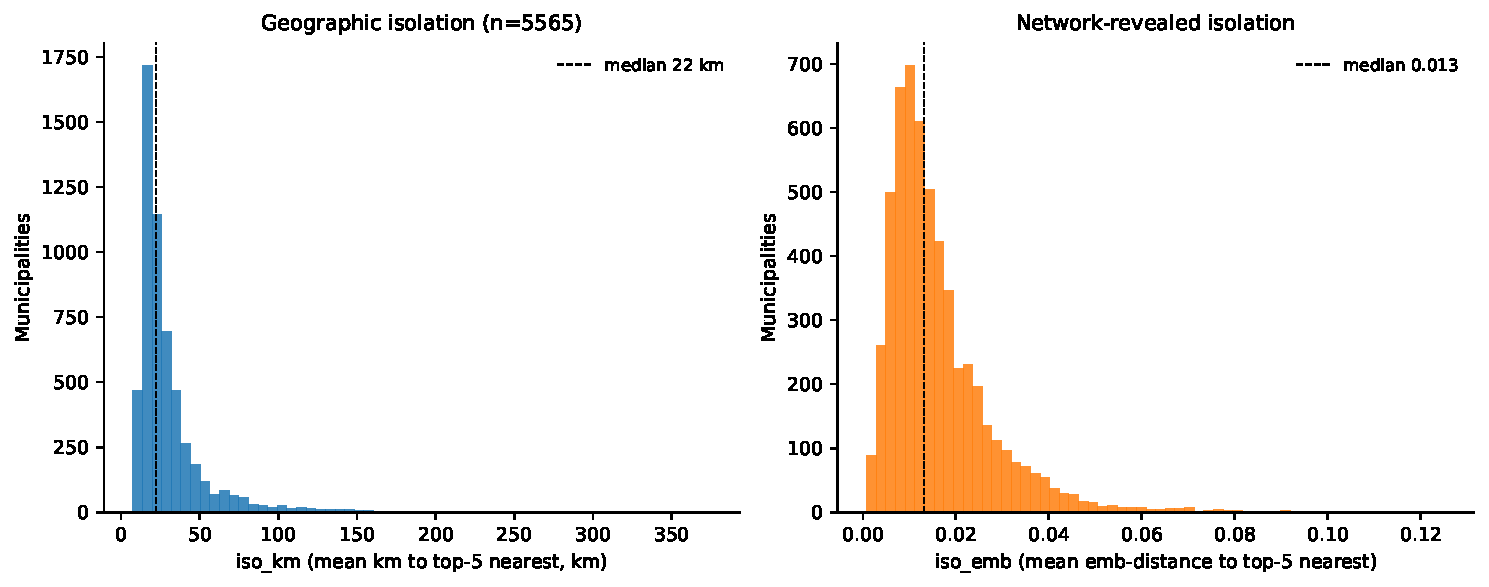
\includegraphics[width=0.92\textwidth]{../04_figures/fig_isolation_distribution.pdf}
    \caption{Cross-sectional distributions of geographic isolation
    (left, in km to nearest high-complexity hospital) and
    embedding-revealed isolation (right, $1 - \cos$ to nearest
    high-complexity hospital in the bipartite embedding). Dashed lines
    indicate medians.}
    \label{fig:iso-distribution}
\end{figure}

\subsection{Side-by-Side Maps of the Two Isolation Measures}

To make the geographical contrast between the two metrics tangible,
Figure \ref{fig:map-side-by-side} shows the spatial distributions of
$\isokm$ (left, in km) and $\isoemb$ (right, in $1 - \cos$). Both
maps share the underlying municipality grid; differences in spatial
texture reflect what each metric captures. The geographic map
darkens uniformly with frontier remoteness in the Amazon basin and
in the cerrado fringe of Mato Grosso. The embedding map shows a
coarser, more clustered structure: high-isolation regions are the
sertão Northeast and pockets of the cerrado, not the Amazon---
because Amazonian patient flow is captured by the embedding through
hospital co-attendance even when the road network is not. The
divergence map of Figure \ref{fig:map-divergence} is, structurally,
the right-minus-left difference (after $z$-scoring).

\begin{figure}[h!]
    \centering
    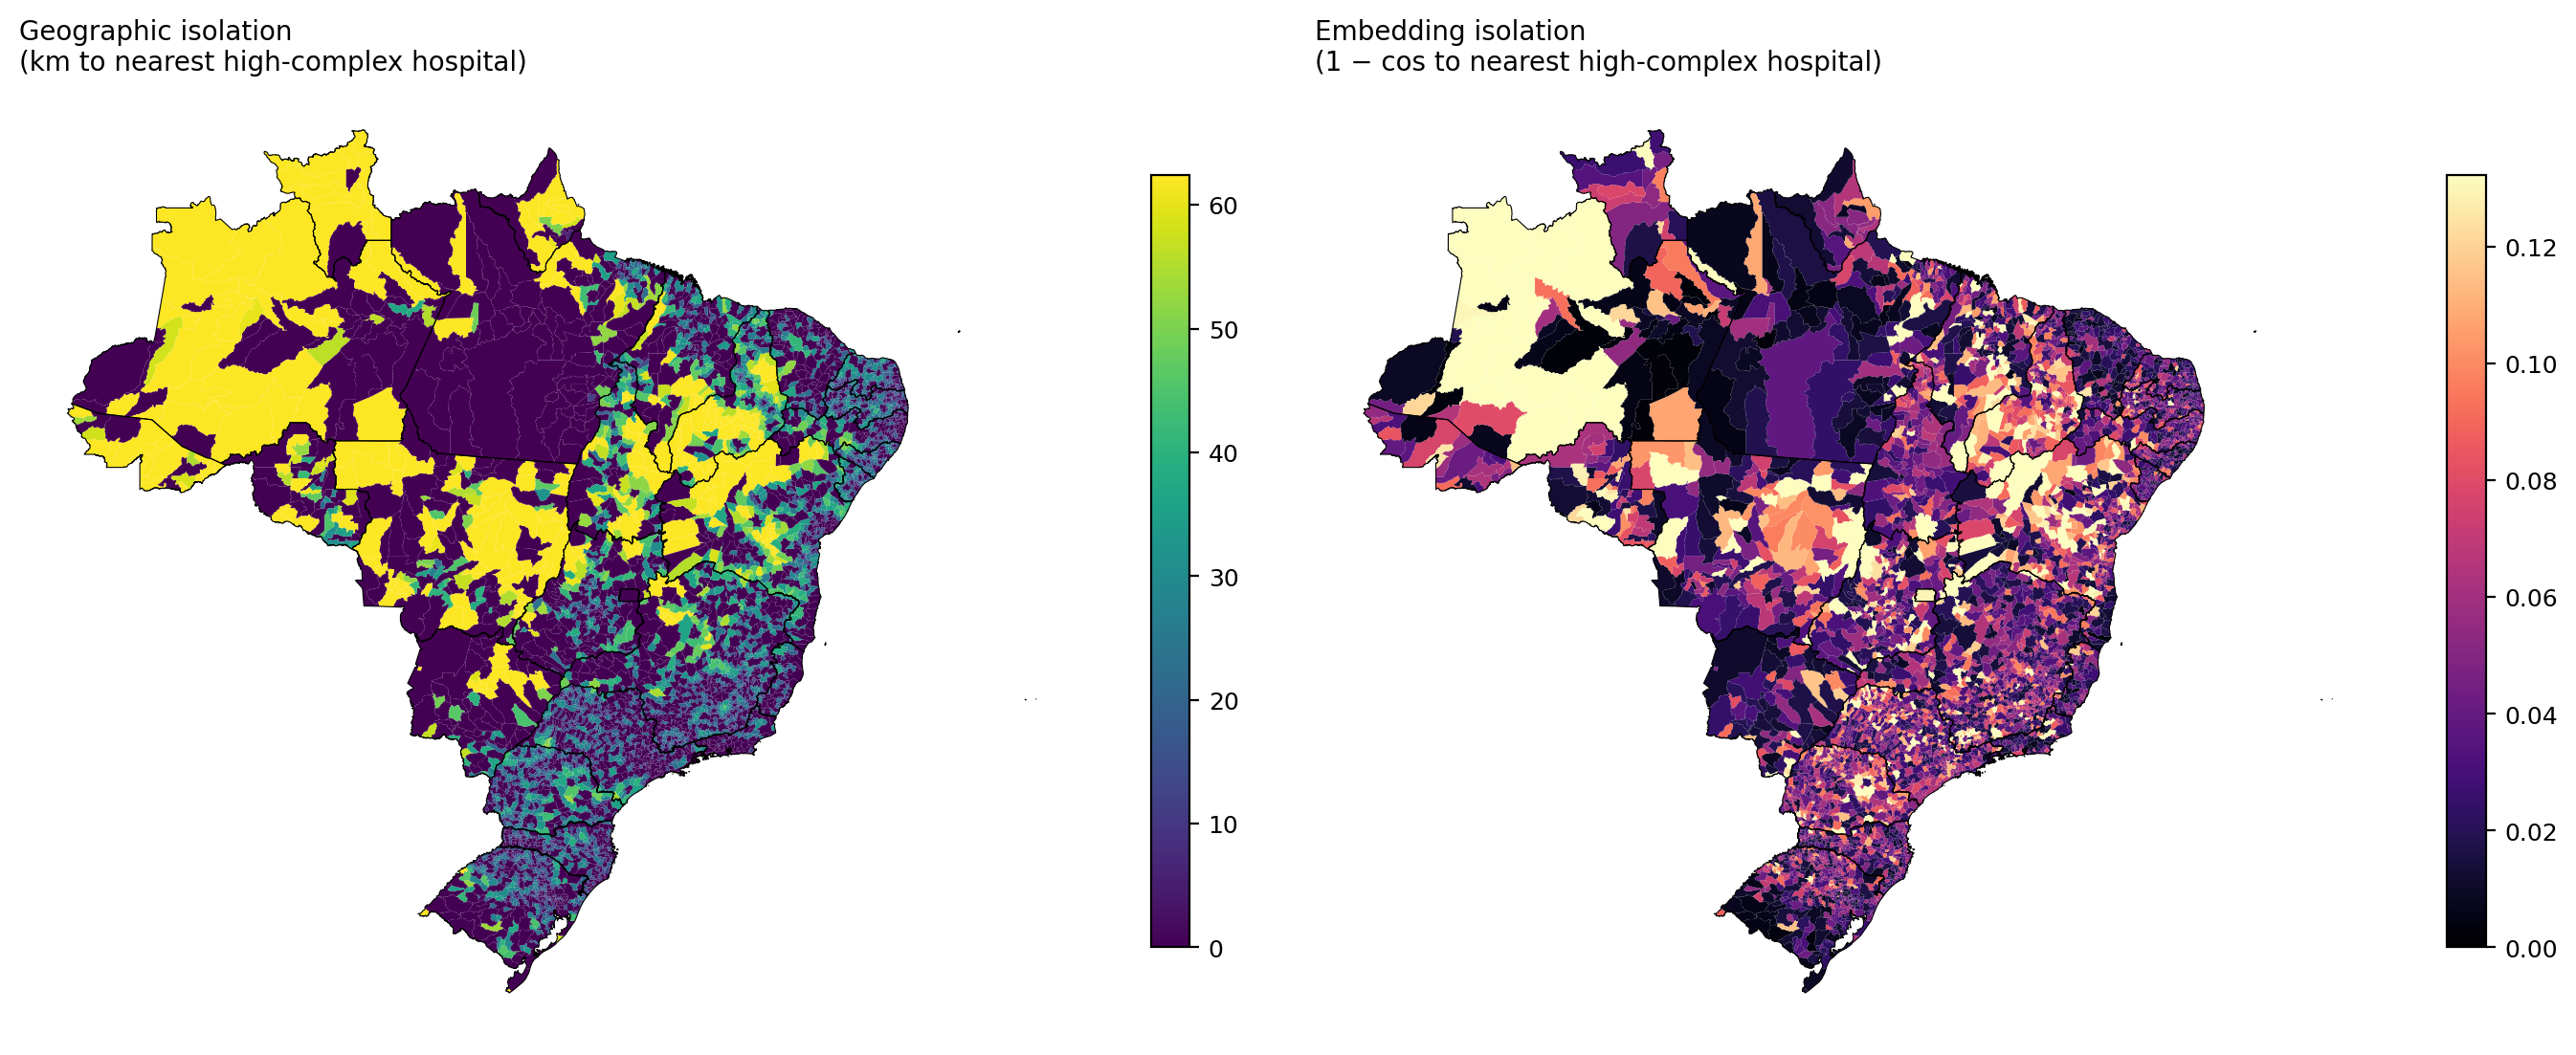
\includegraphics[width=0.99\textwidth]{../04_figures/fig_map_iso_km_vs_emb.png}
    \caption{Side-by-side comparison of geographic isolation (left,
    $\isokm$ in km) and network-revealed isolation (right, $\isoemb$
    as $1 - \cos$). Both maps use sequential perceptually-uniform
    colormaps truncated at the $95$th percentile. Note the divergence
    in the Amazon basin: dark on the geographic map (large km
    distances), but light on the embedding map (active patient flow
    captures the river/air access).}
    \label{fig:map-side-by-side}
\end{figure}

\subsection{Regional and State-Level Patterns}

Table \ref{tab:regional} summarizes the divergence by macro-region.

\begin{table}[h!]
\centering
\caption{Divergence $\divz$ by macro-region.}
\label{tab:regional}
\small
\begin{tabular}{lrrrrrrr}
\toprule
Region & $n$ muns & median $\divz$ & mean $\divz$ & sd & median km & extreme$+$ & extreme$-$ \\
\midrule
Center-West     & 466  & $+0.28$ & $+0.23$ & $1.05$ & 21 &  87 &  54 \\
Southeast       & 1668 & $+0.26$ & $+0.19$ & $0.84$ & 14 & 229 & 151 \\
North           & 449  & $-0.00$ & $-0.22$ & $1.00$ & 29 &  32 & 114 \\
Northeast       & 1794 & $-0.02$ & $-0.12$ & $0.95$ & 19 & 171 & 370 \\
South           & 1188 & $-0.08$ & $-0.10$ & $0.76$ & 14 &  80 & 148 \\
\bottomrule
\end{tabular}
\medskip

\footnotesize
Notes: Median km is the median geographic distance to the nearest
high-complexity hospital, in kilometers. Extreme$+$ (resp. $-$) is the
count of municipalities with $\divz > +1.0$ (resp. $< -1.0$).
\end{table}

The state-level breakdown is reported in Table \ref{tab:uf-ranking},
ordered from least to most calibrated by mean $|\divz|$. Three patterns
stand out.

\begin{table}[ht]
\centering
\caption{State-level miscalibration of the SUS hospital network. States ordered by mean $|\divz|$ (highest = least calibrated). Sign of mean $\divz$ indicates whether the typical municipality in the state is more isolated than km suggests ($+$) or less ($-$). Last column reports the share of the state's municipalities with $|\divz| > 1$.}
\label{tab:uf-ranking}
\small
\setlength{\tabcolsep}{4pt}
\begin{tabular}{llcrrrrrrr}
\toprule
UF & State & Reg & $n$ muns & $\overline{|\divz|}$ & $\overline{\divz}$ & km med & ext$+$ & ext$-$ & ext\% \\
\midrule
  DF & Distrito Federal & CO &     1 & 3.22 & $+$3.22 & 0 &   1 &   0 & 100\% \\
  RR & Roraima & N &    15 & 1.48 & $-$1.26 & 134 &   0 &  10 & 67\% \\
  AC & Acre & N &    22 & 1.21 & $-$1.00 & 81 &   1 &  13 & 64\% \\
  AP & Amap{\'a} & N &    16 & 1.14 & $-$0.87 & 70 &   1 &   9 & 62\% \\
  SE & Sergipe & NE &    75 & 1.11 & $-$0.84 & 19 &   2 &  43 & 60\% \\
  AL & Alagoas & NE &   102 & 1.01 & $-$0.76 & 18 &   4 &  49 & 52\% \\
  TO & Tocantins & N &   139 & 0.91 & $-$0.51 & 36 &   6 &  52 & 42\% \\
  GO & Goi{\'a}s & CO &   246 & 0.87 & $+$0.48 & 19 &  59 &  18 & 31\% \\
  PB & Para{\'i}ba & NE &   223 & 0.86 & $-$0.45 & 16 &  14 &  78 & 41\% \\
  MT & Mato Grosso & CO &   141 & 0.84 & $-$0.15 & 53 &  20 &  27 & 33\% \\
  RN & Rio Grande do Norte & NE &   167 & 0.82 & $-$0.52 & 17 &   2 &  60 & 37\% \\
  MA & Maranh{\~a}o & NE &   217 & 0.75 & $+$0.45 & 20 &  43 &   8 & 24\% \\
  ES & Esp{\'i}rito Santo & SE &    78 & 0.75 & $-$0.07 & 10 &   9 &  16 & 32\% \\
  PI & Piau{\'i} & NE &   224 & 0.73 & $-$0.16 & 39 &  20 &  36 & 25\% \\
  SP & S{\~a}o Paulo & SE &   645 & 0.73 & $+$0.39 & 13 & 126 &  37 & 25\% \\
  PE & Pernambuco & NE &   185 & 0.73 & $-$0.01 & 11 &  15 &  24 & 21\% \\
  BA & Bahia & NE &   417 & 0.70 & $+$0.25 & 23 &  67 &  28 & 23\% \\
  PR & Paran{\'a} & S &   399 & 0.68 & $+$0.08 & 19 &  47 &  40 & 22\% \\
  MG & Minas Gerais & SE &   853 & 0.67 & $+$0.03 & 17 &  80 &  94 & 20\% \\
  MS & Mato Grosso do Sul & CO &    78 & 0.66 & $+$0.08 & 0 &   7 &   9 & 21\% \\
  SC & Santa Catarina & S &   293 & 0.65 & $-$0.11 & 11 &  22 &  36 & 20\% \\
  RJ & Rio de Janeiro & SE &    92 & 0.65 & $+$0.43 & 0 &  14 &   4 & 20\% \\
  AM & Amazonas & N &    62 & 0.64 & $+$0.19 & 47 &   9 &   6 & 24\% \\
  CE & Cear{\'a} & NE &   184 & 0.64 & $-$0.25 & 0 &   4 &  44 & 26\% \\
  PA & Par{\'a} & N &   143 & 0.63 & $+$0.07 & 0 &  12 &  21 & 23\% \\
  RS & Rio Grande do Sul & S &   496 & 0.58 & $-$0.22 & 13 &  11 &  72 & 17\% \\
  RO & Rond{\^o}nia & N &    52 & 0.52 & $+$0.13 & 32 &   3 &   3 & 12\% \\
\bottomrule
\end{tabular}
\medskip

\footnotesize
Notes: $\overline{|\divz|}$ is the mean of the unsigned divergence $z$-score; higher means the state's municipalities deviate more from geographic prediction in either direction. $\overline{\divz}$ is the signed mean; ext$+$ (resp. ext$-$) counts municipalities with $\divz > 1$ (resp.\ $< -1$). km med is the median geographic distance to the nearest high-complexity hospital, in kilometers.
\end{table}


First, the four Northern states with frontier geography---Roraima,
Acre, Amapá, plus Tocantins---occupy the top ranks alongside the
narrow-coastal Northeast (Sergipe, Alagoas, Paraíba, Rio Grande do
Norte). All exhibit signed-mean divergences that are \emph{negative},
indicating that km systematically overstates isolation in these states.
The mechanism differs across the two clusters: river and air
connections in the Amazonian frontier, and informal cross-border
referral flows toward Salvador, Recife, and Aracaju in the Northeast.

Second, only two of the top-ten miscalibrated states have a positive
signed mean: the Distrito Federal ($+3.22$, but $n = 1$ and an outlier
case in which the federal capital itself is bypassed for services in
Goiás) and Goiás ($+0.48$), the latter reflecting absorption of
referrals from neighboring states into the Brasília tertiary
infrastructure. The asymmetry is striking: the most miscalibrated
systems in Brazil are predominantly those where geographic distance
overstates isolation---a sign that informal access channels carry
considerable patient load.

Third, Rondônia is the best-calibrated state in our panel
($\overline{|\divz|} = 0.52$, only $12\%$ of municipalities with
$|\divz| > 1$), despite being part of the Amazonian frontier. The
mature consolidation of Porto Velho's tertiary hospitals and the
predominance of paved BR-364 connections explain the alignment.

\subsection{Cross-Sectional Mortality: A Predictive Null}
\label{sec:results-mortality}

We turn finally to the question of whether the divergence---or its
underlying components $\isokm$ and $\isoemb$---predicts amenable
mortality conditional on standard controls. Table \ref{tab:cv-mortality}
reports the $5$-fold cross-validated $R^2$ and MAE for a sequence of
ridge specifications.

\begin{table}[h!]
\centering
\caption{Out-of-sample $R^2$ for amenable mortality regressions, ridge with $5$-fold CV.}
\label{tab:cv-mortality}
\small
\begin{tabular}{lcccc}
\toprule
Specification & $R^2$ & SD & MAE & $\Delta R^2$ vs km \\
\midrule
$M_0$: pop $+$ GDP $+$ UF FE                  & $0.392$ & $0.056$ & $26.5$ & --       \\
$M_{km}$: $M_0 + z(\log\isokm)$               & $0.405$ & $0.055$ & $26.0$ & --       \\
$M_{emb}$: $M_0 + z(\isoemb)$                 & $0.397$ & $0.054$ & $26.3$ & $-0.009$ \\
$M_{both}$: $M_0 + z(\log\isokm) + z(\isoemb)$ & $0.405$ & $0.055$ & $26.0$ & $-0.000$ \\
$M_{|\divz|}$: $M_0 + |\divz|$                & $0.392$ & $0.055$ & $26.5$ & $-0.013$ \\
$M_{km + |\divz|}$: $M_0 + z(\log\isokm) + |\divz|$ & $0.406$ & $0.056$ & $26.0$ & $+0.001$ \\
\bottomrule
\end{tabular}
\medskip

\footnotesize
Notes: Sample is $n = 3{,}112$ municipalities with mean population $\geq
10{,}000$, $2010\text{--}2023$. Outcome is the period-pooled amenable
mortality rate per $100{,}000$, winsorized at $[1\%, 99\%]$. Ridge
penalty $\alpha = 1$, random seed $42$.
\end{table}

The descriptive observation is unambiguous: \emph{the embedding does
not predict amenable mortality} once standard controls and geographic
distance are included. $M_0$ alone explains $39.2\%$ of out-of-sample
variance; adding geographic isolation yields a $1.3$ percentage-point
gain ($M_{km}$); adding embedding-isolation alone is dominated by
geographic isolation ($M_{emb}$ vs $M_{km}$: $\Delta R^2 = -0.009$);
combining the two is statistically indistinguishable from
$M_{km}$. Replacing the embedding with the divergence
metric---$|\divz|$ or its signed split---produces the same null result.

We argue this null is informative, but in a different direction than
one might initially read it. We discuss the interpretation in Section
\ref{sec:discussion}.
